\documentclass[11pt,titlepage]{article}
\usepackage[margin=1in]{geometry}
\usepackage[T1]{fontenc}
\usepackage{graphicx}
\usepackage{booktabs}
\usepackage{amsmath}
\usepackage[hidelinks]{hyperref}

\title{CSC311 Machine Learning Project: Proposal}
\author{Zhaoning Zhang\and Luhan Ma \and Adish Singh \and Jingtian Hu \and Group: 63376}
\date{Fall 2026}

\begin{document}
\maketitle

% All numbers in this document are printed by code.py (seed 311; see
% output.txt in code.zip) and are computed on the training split only.
% Keep figures/figure.png next to this file.

\section{Data Exploration}\label{sec:data-exploration}

\paragraph{Basic Overview.}
The dataset has 870 responses from 290 students, each answering the same 12 questions once per sport (290 rows per class). We split by student, not by row, because a student’s three rows share an answering style and a row-level split would leak information. The id is not a feature: test ids never occur in training, so it could only help memorize individuals. Before exploring, we held out 15\% of students (44 students, 132 rows, seed 311; Appendix A) as a test set. Everything below uses the remaining 246 students (738 rows).

\begin{table}[h]
\centering\footnotesize
\begin{tabular}{@{}llrl@{}}
\toprule
Feature & Type & Missing & Representation\\
\midrule
Ease of starting   & numeric 0--10      & 2  & standardized; median imputation        \\
Strategy           & Likert (5 levels)  & 3  & ordinal 1--5, standardized             \\
Injury risk        & Likert (5 levels)  & 2  & ordinal 1--5, standardized             \\
Individual $>$ team & Likert (5 levels)  & 3  & ordinal 1--5, standardized            \\
Where played       & multi-select (7)   & 2  & 7 binary indicators                    \\
Season             & multi-select (4)   & 2  & 4 binary indicators                    \\
Music              & multi-select (10)  & 2  & 10 binary indicators                   \\
Food \& drink      & free text          & 15 & bag of words (120 tokens)              \\
Colour             & free text          & 6  & bag of words (22 tokens)               \\
Song               & free text          & 62 (81) & bag of words (145 tokens)         \\
Feeling            & free text          & 3  & bag of words (178 tokens)              \\
Price              & free text $\to$ number & 6 (32) & $\log(1+p)$, median imputation, flag \\
\bottomrule
\end{tabular}
\caption{Features on the training split (738 rows). Missing = blank answers; parentheses include song placeholders and unparseable prices.}
\label{tab:features}
\vspace{-1em}
\end{table}

\paragraph{Distributions and patterns.}
Figure~\ref{fig:eda} compares the non-text features across sports.
\textbf{(a)} Baseball is rated harder to start (mean 4.03) than Basketball (6.08)
or Soccer (6.19), which separates Baseball but not Basketball from Soccer.
\textbf{(b)} Likert answers show the same split: 28\% of Baseball responses agree
that the injury risk is high, against about 70\% for the others; the
``individual brilliance'' statement instead isolates Soccer (33\% agree versus
65\% and 63\%).
\textbf{(c)} Baseball has a lower median price (\$52.50 versus \$150 for Basketball
and \$175 for Soccer), with heavy overlap.
In the text fields, the most frequent tokens are class specific: colour
(\emph{blue}/\emph{orange}/\emph{green} for Baseball/Basketball/Soccer), song
(\emph{Take Me Out to the Ball Game}, Drake, \emph{Waka Waka}), and food
(\emph{hot dogs} for Baseball, wings for Basketball). Feeling separates Baseball
(\emph{bored} in 26\% of its rows versus \emph{excited} in 10\%) but not Basketball
from Soccer (\emph{excited} in 37\% versus 40\%).

\paragraph{Near-constant and correlated features.}
A feature that is almost always the same tells the model little, and highly
correlated features make a linear model's weights unstable. Neither is a problem
here: every multi-select option is chosen in 3--92\% of rows, and the Likert and
ease features are weakly correlated (Spearman $|\rho| \leq 0.33$). Only rare
tokens are near-constant, and we drop them (see Preprocessing).

\begin{figure}[t]
\centering
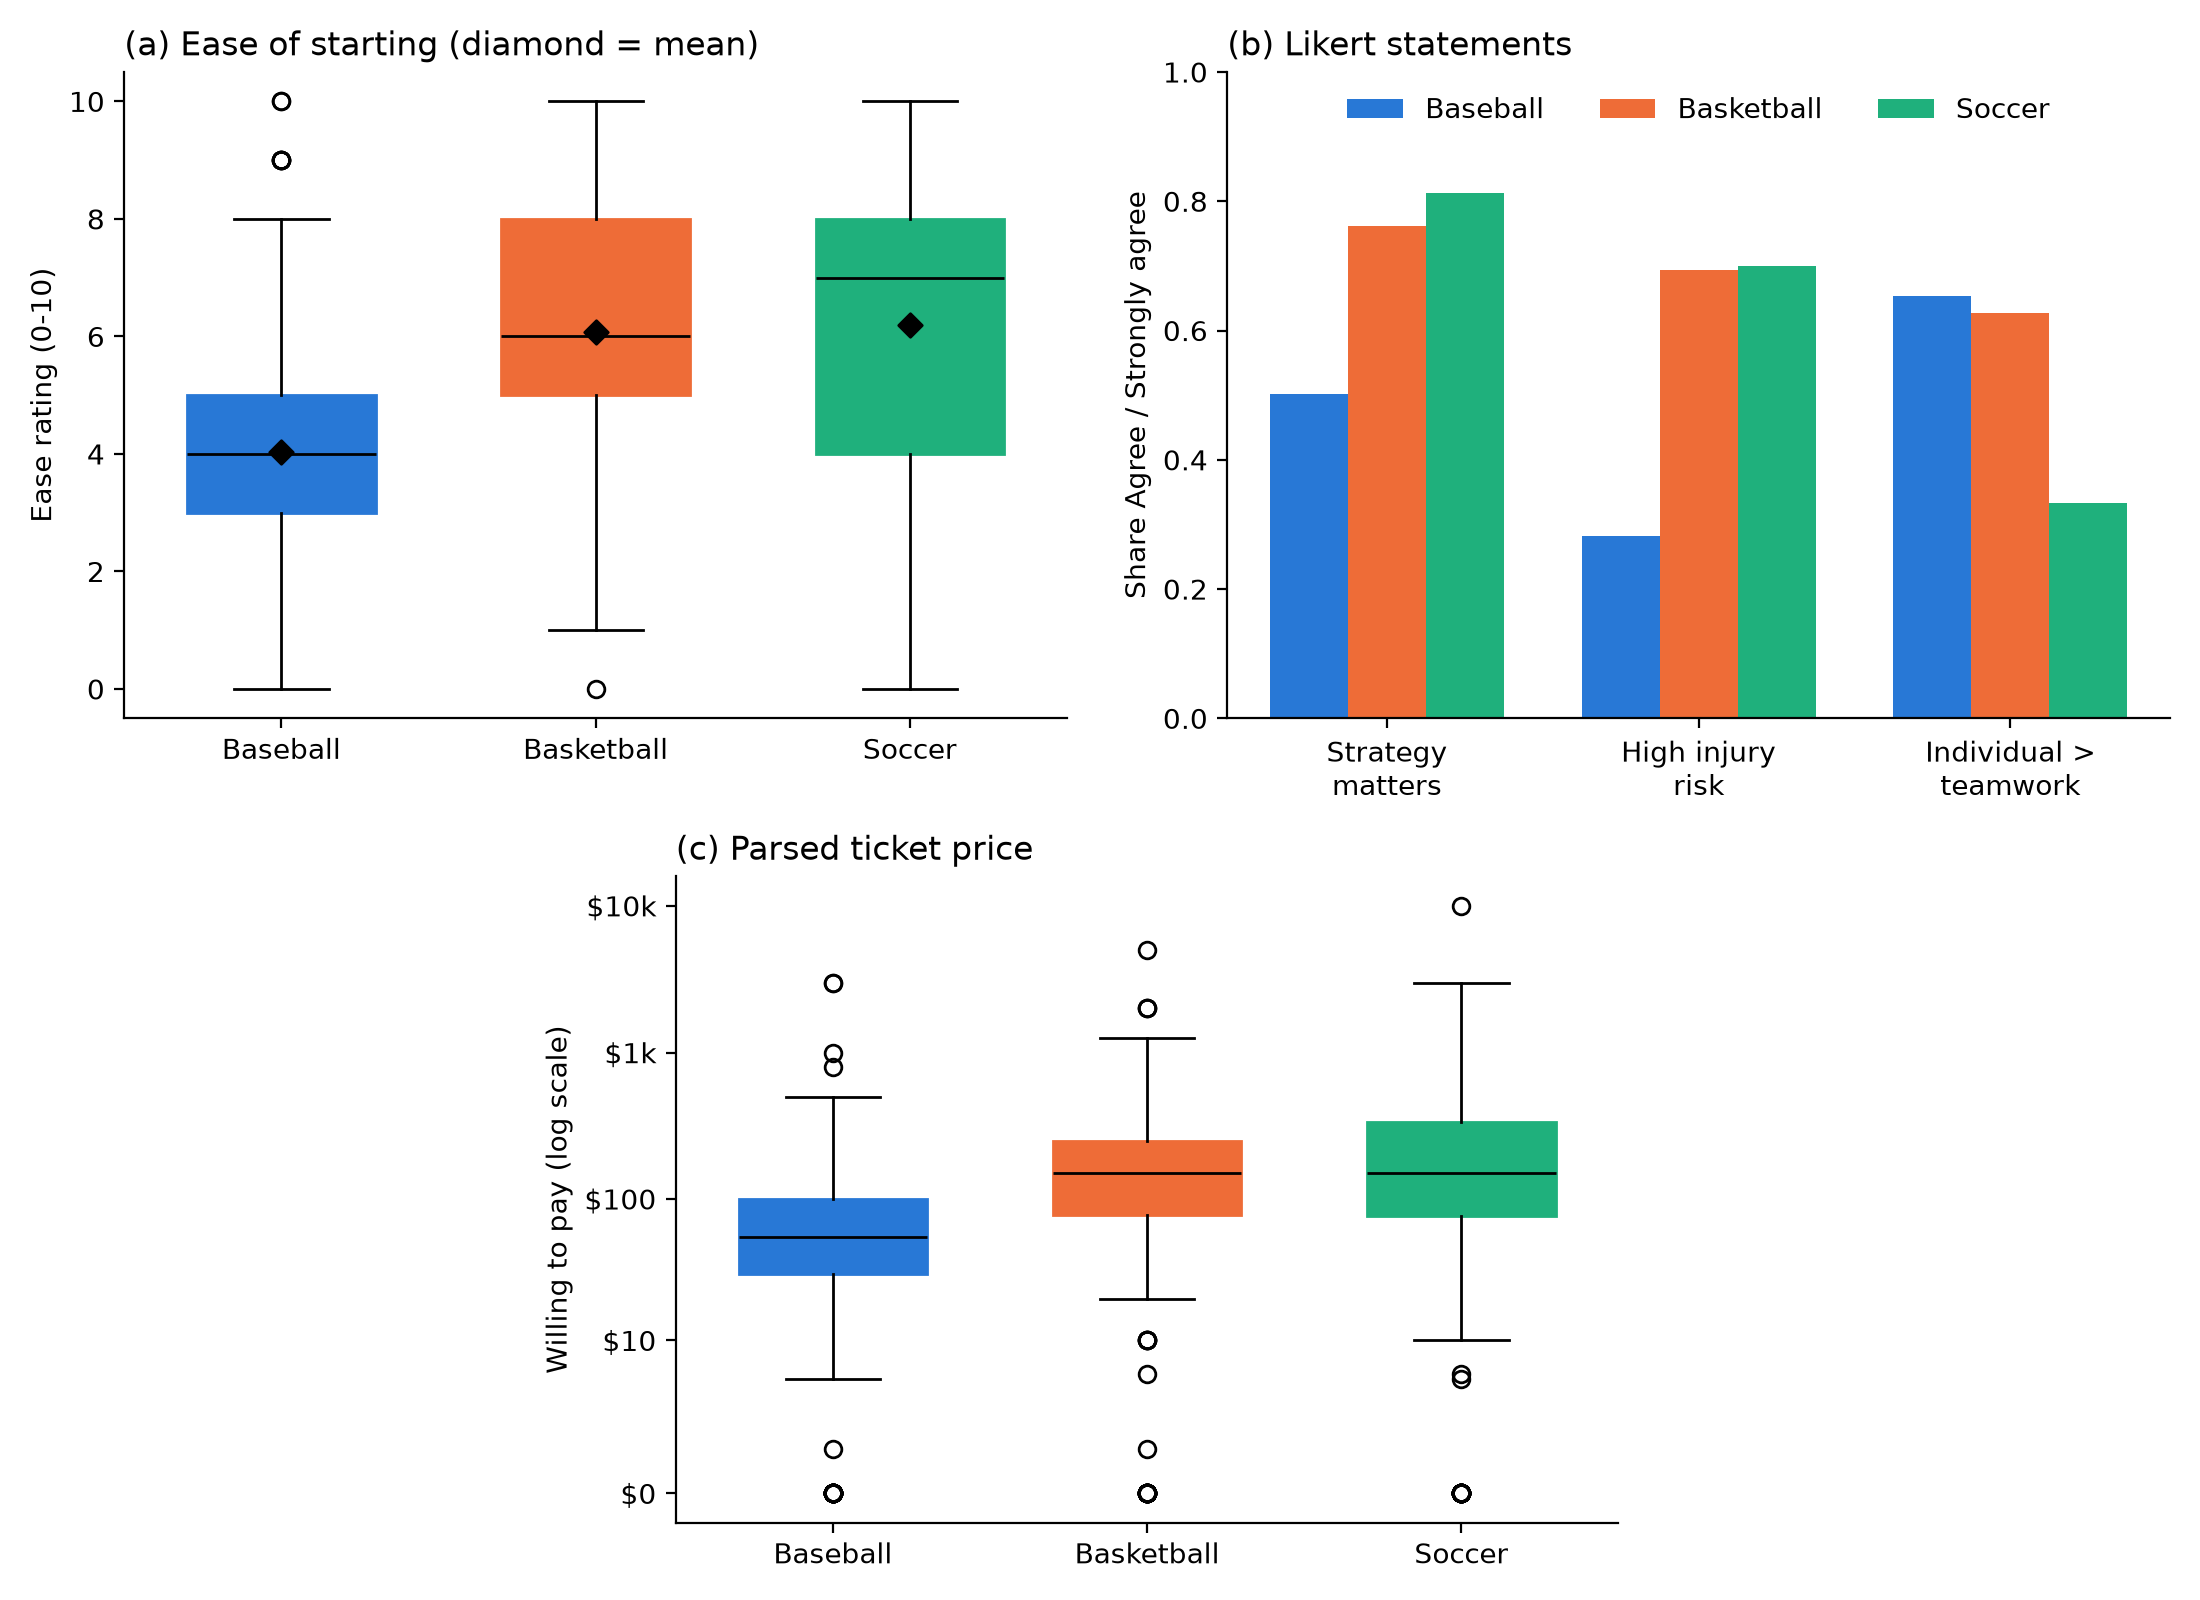
\includegraphics[width=0.65\linewidth]{figures/figure.png}
\caption{Training split, by sport. (a) Ease rating. (b) Share agreeing with each
Likert statement. (c) Parsed ticket price on a $\log(1+p)$ scale.}
\label{fig:eda}
\vspace{-1em}
\end{figure}

\paragraph{Missing values, outliers, and inconsistencies.}
\begin{itemize}\itemsep0pt
\item \textbf{Missing values:} rare (at most 6 rows per feature) except food (15)
and song (62, 8.4\%), plus 19 song placeholders (``none'', ``idk'', ``-'') that we
also count as missing. Song is likely skipped when none comes to mind. Missingness
depends on the label: song is blank in 11\% of Baseball and Basketball rows but 3\%
of Soccer rows, and food is never missing for Soccer. A missing answer is therefore
a signal, so we keep it as an empty bag of words instead of imputing it.
\item \textbf{Text fields:} normalizing capitalization, punctuation, and
non-breaking spaces reduces 189 distinct colour answers to 122. Typos
(\emph{exited} for \emph{excited}) remain, and 58--63\% of the tokens in each field
occur only once; the rare-token filter in Preprocessing removes most of them.
\item \textbf{Price:} 280 distinct strings mix units (``150CAD''), separators
(``\$10\,000''), ranges, and sentences. Our regex parser reads 634 single
numbers, 39 range midpoints, and 33 refusals (``Zero'') as \$0, and treats 26
unparseable answers as missing. Price is right-skewed (median \$100, max
\$10{,}000), so we apply $\log(1+p)$ rather than delete plausible answers,
ignoring the small USD/CAD difference.
\end{itemize}

\paragraph{Preprocessing and its justification.}
\begin{itemize}\itemsep0pt
\item \textbf{Numeric and Likert:} median imputation; Likert answers become
integers 1--5 rather than one-hot vectors because the levels are ordered and the
class differences monotone (Figure~\ref{fig:eda}b). These and log-price are
standardized to match the scale of the binary features under L2 regularization; a
flag marks unparseable prices.
\item \textbf{Multi-select:} one binary indicator per option (empty answer = all
zeros). Treating each combination as a category would create 58, 13, and 99 sparse
categories and hide shared options (82\% of responses listing Winter are
Basketball).
\item \textbf{Text:} normalize to lowercase, replace non-breaking spaces, strip punctuation, and
remove a short stop-word list (\emph{and}, \emph{the}, \emph{by} were frequent in
every class). Each field gets its own binary bag-of-words vocabulary, since the same
word can mean different things in different questions. To limit the number of
features relative to our 738 rows, tokens that appear in fewer than $m$ training
rows are dropped, removing most typos and one-off answers. This section uses
$m = 3$ (465 text features remain); $m$ is tuned in Section~\ref{sec:methodology}.
If we have extra time, we will optimize this text feature using averaged pre-trained word
embeddings (Section~\ref{sec:methodology}).

\end{itemize}
\textbf{No leakage:} all fitted quantities (medians, means, variances,
vocabularies) come from the training data only, and from the training folds only
inside cross-validation.
% ===============================================================

\section{Methodology}\label{sec:methodology}

\paragraph{Model families and why they suit the data.}
We compare three model families, chosen from the findings above and from the
constraint that the final \texttt{pred.py} may use only NumPy and pandas. From our Data Exploration we expect the most predictive features to be ease of starting, injury-risk agreement, and the colour, song and food tokens.
\begin{enumerate}\itemsep0pt
\item \textbf{Multinomial logistic regression (LR).} Our features are mostly sparse
binary indicators and tokens, each of which shifts the evidence toward one class
roughly independently (Section~\ref{sec:data-exploration}). A linear model is a
natural fit, is interpretable through its weights, and is unlikely to overfit with
L2 regularization on 738 rows. It is our baseline.
\item \textbf{Random forest (RF).} Class differences in our Data Exploration are threshold-like (Baseball has low ease ratings and low injury-risk agreement), and a missing song or food answer is itself informative. Trees split on these directly and can combine tokens (e.g. “orange” with “wings”) without hand-built interactions. Averaging many trees reduces the high variance of a single tree.
\item \textbf{Multilayer perceptron (MLP).} A one- or two-hidden-layer network can
learn nonlinear combinations of all features, including dense word-embedding
features. We include it to test whether extra capacity helps; given the small
dataset, it requires strong regularization.
\end{enumerate}

\paragraph{Training setup.}
Training uses Python with \texttt{numpy}, \texttt{scikit-learn}, and
\texttt{pandas}; all random seeds are fixed to 311. The preprocessing of
Section~\ref{sec:data-exploration} is implemented as a single pipeline that is
refitted on the training portion of every split.
\begin{itemize}\itemsep0pt
\item \textbf{LR:} softmax output with cross-entropy loss and an L2 penalty of
strength $1/C$, optimized with L-BFGS (scikit-learn's \texttt{lbfgs} solver) for
up to 5000 iterations or until the gradient tolerance $10^{-4}$ is met. The loss is
convex, so L-BFGS converges to the global minimum and no learning rate or early
stopping is needed.
\item \textbf{RF:} Each tree is grown greedily on a
bootstrap sample using the Gini impurity, considering a random subset of features
at each split. There is no gradient-based optimizer; regularization comes from
limiting depth and leaf size and from averaging the trees.
\item \textbf{MLP:} ReLU hidden layers, softmax output, cross-entropy loss with L2
weight penalty $\alpha$, optimized with Adam (scikit-learn defaults
$\beta_1 = 0.9$, $\beta_2 = 0.999$) on mini-batches of 32 with a constant learning
rate. For early stopping we hold out 10\% of the \emph{students} of the current
training fold, train epoch by epoch (\texttt{partial\_fit}), stop after 20 epochs
without improvement in validation loss (maximum 500 epochs), and restore the
weights from the best epoch. Holding out students rather than rows prevents the
same leakage described in Section~\ref{sec:data-exploration}. When the final MLP is
retrained on all training students, the same 10\% student holdout is used for early
stopping.
\end{itemize}

\paragraph{Validation strategy.}
The 44-student test set is untouched during this stage. On the 246 training
students we run 5-fold cross-validation grouped by student
(\texttt{GroupKFold} on \texttt{id} after shuffling the ids with seed 311): each fold
holds out about 49 students (about 147 rows), and the three rows of a student are
always in the same fold. Because every student answers once per sport, each fold
is exactly balanced across the three classes without explicit stratification.
All models and all hyperparameter settings are evaluated on
the \emph{same} five folds, so their scores are directly comparable. A setting's
score is its mean validation metric over the five folds, and we also report the
standard deviation across folds to show how much of a difference is noise.

\paragraph{Hyperparameter search.}
Table~\ref{tab:hparams} lists the hyperparameters and ranges. For LR we use a full
grid search, since there are only two hyperparameters ($C$ and $m$; 24 settings).
For RF and MLP we use random
search with 60 sampled configurations each, which covers wide ranges at the same
budget for both models (log-uniform sampling for $\alpha$ and the learning rate).
The minimum token count $m$ is tuned jointly with each model because it controls
the number of features. The selection criterion is mean cross-validated
accuracy; when two settings are within one standard error of the best one (the
standard deviation of the best setting's five fold scores divided by $\sqrt{5}$), we
pick the simpler one (larger $1/C$, smaller forest or network).

\begin{table}[h]
\centering\small
\begin{tabular}{@{}lll@{}}
\toprule
Model & Hyperparameter & Values / range\\
\midrule
All & min.\ token count $m$ & $\{2, 3, 5, 10\}$\\
\midrule
LR  & inverse regularization $C$ & $\{10^{-3}, 10^{-2}, \dots, 10^{2}\}$ (6 values, log grid)\\
\midrule
RF  & number of trees & $\{100, 200, 300, 500\}$\\
    & max.\ depth & $\{5, 10, 15, 20, \text{none}\}$\\
    & min.\ samples per leaf & $\{1, 2, 4, 8\}$\\
    & features per split & $\{\sqrt{d},\ \log_2 d,\ 0.2d\}$\\
\midrule
MLP & hidden layers & $\{(32), (64), (128), (64, 32)\}$\\
    & L2 penalty $\alpha$ & $[10^{-5}, 10^{-1}]$, log-uniform\\
    & learning rate & $[10^{-4}, 10^{-2}]$, log-uniform\\
\bottomrule
\end{tabular}
\caption{Hyperparameters and search ranges. $d$ is the number of input features.}
\label{tab:hparams}
\end{table}

To show that the ranges are reasonable, we will plot the mean validation accuracy
(with a $\pm$1 standard deviation band) against the most important hyperparameter
of each model ($C$ for LR, maximum depth for RF, $\alpha$ for the MLP), together
with the training accuracy. We check that the best value lies inside the range,
not at its edge (otherwise we extend the range), and use the gap between training
and validation accuracy to judge under- or overfitting.

\paragraph{Fair comparison.}
Every model family is tuned with the procedure above \emph{before} the families are
compared. The comparison uses each family's best configuration and its
cross-validated scores on the shared folds; we never pick a family based on its
default hyperparameters.

\paragraph{Additional experiment: text representation.}
Because the test respondents may use words not seen in training, we compare two
text representations for the tuned LR and MLP: (i) bag of words only, and
(ii) bag of words plus, for each text field, the average of 50-dimensional GloVe
vectors (\texttt{glove.6B.50d}) of its tokens, with unknown tokens skipped and an
all-zero vector if no token is known. To meet the 10\,MB submission limit, we keep
the vectors of the 20{,}000 most frequent English words, stored as 16-bit floats
(about 2\,MB). Representation (ii) is kept only if it improves cross-validated
accuracy beyond one standard error.

\paragraph{Evaluation metrics.}
\begin{itemize}\itemsep0pt
\item \textbf{Accuracy} is the main selection metric. The classes are exactly
balanced, so accuracy is not biased toward a majority class, and it is the
quantity on which the test set is graded.
\item \textbf{Macro-averaged F1, with per-class precision and recall.} Accuracy can
hide one weak class. Section~\ref{sec:data-exploration} suggests that Basketball
and Soccer are harder to separate from each other than from Baseball (similar ease
ratings and Likert answers), so we track per-class recall to detect this.
\item \textbf{Confusion matrix} of the pooled out-of-fold predictions, to identify
the most common misclassifications and inspect examples of them.
\end{itemize}
All metrics are reported as mean $\pm$ standard deviation over the five folds.

\paragraph{Final model and test estimate.}
We select the family and configuration with the best cross-validated accuracy, using
the one-standard-error rule in favour of the simpler model. We then retrain it on
all 738 training rows, evaluate it exactly once on the 132-row test set, and report
that accuracy as our estimate of performance on unseen data, with a 95\% confidence
interval from 1000 bootstrap resamples of the 44 test students. With only 132 rows
this interval is wide (about $\pm 5$ points at 90\% accuracy), and because the real
test set comes from TAs and instructors rather than students, the estimate may be
optimistic. After this single evaluation, we retrain the chosen configuration on
all 870 rows for \texttt{pred.py}. We export the fitted preprocessing (medians,
means and variances, vocabularies) and model parameters (LR or MLP weight matrices,
or the RF trees as arrays of split features, thresholds, child indices, and leaf
class probabilities) to a compressed \texttt{.npz} file, with the vocabularies in a
small \texttt{.json} file. Storing trees as compact binary arrays matters for the
10\,MB limit: 500 fully grown trees take under 1\,MB this way but 5--9\,MB as JSON.
We then reimplement the prediction step in NumPy and verify that it reproduces the
trained results exactly on the validation folds.

% ===============================================================

\section*{Use of AI Tools}
We used Claude (Anthropic) for three purposes: revising our hand-written draft for
clarity; checking every number in this proposal against the output of
\texttt{code.py}; estimating the export size of a random forest, which
informed our choice of file format. We reviewed every change and take
responsibility for the content.
% ===============================================================

\appendix
\section{Held-out Test Set}\label{app:test-ids}
The test set consists of the following 44 student ids (132 rows), drawn uniformly
at random without replacement from ids 1--290 with
\texttt{numpy.random.default\_rng(311)}. The training set consists of the other
246 ids (738 rows).

\medskip
\noindent\small
6, 13, 15, 16, 17, 18, 22, 31, 35, 38, 42, 49, 58, 69, 77, 82, 84, 87, 90, 94, 103, 113, 119, 141, 152, 158, 162, 168, 178, 180, 190, 200, 206, 218, 258, 261, 262, 266, 276, 279, 281, 282, 283, 287.
\normalsize

\end{document}
